%保存为UTF-8编码格式
%用xelatex编译
 
\documentclass[UTF8,a4paper,12pt]{ctexart}
\usepackage[left=2cm, right=2cm, top=2cm, bottom=2cm]{geometry} %页边距
\CTEXsetup[format={\Large\bfseries}]{section} %设置章标题字号为Large,居左
%\CTEXsetup[number={\chinese{section}}]{section}
%\CTEXsetup[name={(,)}]{subsection}
%\CTEXsetup[number={\chinese{subsection}}]{subsection}
%\CTEXsetup[name={(,)}]{subsubsection}
%\CTEXsetup[number=\arabic{subsubsection}]{subsubsection}  %以上四行为各级标题样式设置,可根据需要做修改
 
\linespread{1.5} %设置全文行间距
 
 
%\usepackage[english]{babel}
%\usepackage{float}     %放弃美学排版图表
\usepackage{fontspec}   %修改字体
\usepackage{amsmath, amsfonts, amssymb} % 数学公式相关宏包
\usepackage{color}      % color content
\usepackage{graphicx}   % 导入图片
\usepackage{subfigure}  % 并排子图
\usepackage{url}        % 超链接
\usepackage{bm}         % 加粗部分公式,比如\bm{aaa}aaa
\usepackage{multirow}
\usepackage{booktabs}
\usepackage{epstopdf}
\usepackage{epsfig}
\usepackage{longtable}  %长表格
\usepackage{supertabular}%跨页表格
\usepackage{algorithm}
\usepackage{algorithmic}
\usepackage{changepage}
\usepackage{caption}
\usepackage[dvipsnames]{xcolor} % 更全的色系
\usepackage{listings} % 排代码用的宏包
 
\lstset{
	basicstyle          =   \small\ttfamily,          % 基本代码风格
	keywordstyle        =   \bfseries,          % 关键字风格
	commentstyle        =   \rmfamily\itshape,  % 注释的风格,斜体
	stringstyle         =   \ttfamily,  % 字符串风格
	flexiblecolumns,                % 别问为什么,加上这个
	numbers             =   left,   % 行号的位置在左边
	showspaces          =   false,  % 是否显示空格,显示了有点乱,所以不现实了
	numberstyle         =   \zihao{-5}\ttfamily,    % 行号的样式,小五号,tt等宽字体
	showstringspaces    =   false,
	captionpos          =   t,      % 这段代码的名字所呈现的位置,t指的是top上面
	frame               =   lrtb,   % 显示边框
}
 
%%%%%%%%%%%%%%%%%%%%%%%
% -- text font --
% compile using Xelatex
%%%%%%%%%%%%%%%%%%%%%%%
% -- 中文字体 --
%\setCJKmainfont{Microsoft YaHei}  % 微软雅黑
%\setCJKmainfont{YouYuan}  % 幼圆
%\setCJKmainfont{NSimSun}  % 新宋体
%\setCJKmainfont{KaiTi}    % 楷体
\setCJKmainfont{SimSun}   % 宋体
%\setCJKmainfont{SimHei}   % 黑体
 
% -- 英文字体 --
\setmainfont{Times New Roman}
%\setmainfont{DejaVu Sans}
%\setmainfont{Latin Modern Mono}
%\setmainfont{Consolas}
%
%
\renewcommand{\algorithmicrequire}{ \textbf{Input:}}     % use Input in the format of Algorithm
\renewcommand{\algorithmicensure}{ \textbf{Initialize:}} % use Initialize in the format of Algorithm
\renewcommand{\algorithmicreturn}{ \textbf{Output:}}     % use Output in the format of Algorithm
\renewcommand{\abstractname}{\textbf{\large {摘\quad 要}}} %更改摘要二字的样式
\newcommand{\xiaosi}{\fontsize{12pt}{\baselineskip}}     %\xiaosi代替设置12pt字号命令,不加\selectfont,行间距设置无效
\newcommand{\wuhao}{\fontsize{10.5pt}{10.5pt}\selectfont}
 
\usepackage{fancyhdr} %设置全文页眉、页脚的格式
\pagestyle{fancy}
\lhead{}           %页眉左边设为空
\chead{}           %页眉中间
\rhead{}           %页眉右边
%\rhead{\includegraphics[width=1.2cm]{1.eps}}  %页眉右侧放置logo
\lfoot{}          %页脚左边
\cfoot{\thepage}  %页脚中间
\rfoot{}          %页脚右边
 
 
%%%%%%%%%%%%%%%%%%%%%%%
%  设置水印
%%%%%%%%%%%%%%%%%%%%%%%
%\usepackage{draftwatermark}         % 所有页加水印
%\usepackage[firstpage]{draftwatermark} % 只有第一页加水印
% \SetWatermarkText{Water-Mark}           % 设置水印内容
% \SetWatermarkText{\includegraphics{fig/ZJDX-WaterMark.eps}}         % 设置水印logo
% \SetWatermarkLightness{0.9}             % 设置水印透明度 0-1
% \SetWatermarkScale{1}                   % 设置水印大小 0-1
 
\usepackage{hyperref} %bookmarks
\hypersetup{colorlinks, bookmarks, unicode} %unicode
 
 
 
\title{\textbf{\Large{第三次小作业:图像复原任务 报告}}}
\author{涂宇清}
\date{522030910152}
 
 
 
\begin{document}
 
\maketitle
%\tableofcontents
\setcounter{page}{1}        %从下面开始编页,页脚格式为导言部分设置的格式
 
 
\section{DeepPermNet网络构建}
采用DeepPermNet网络结构。其接受一连串图像输入,每个图像均经过一个共享权重的AlexNet,然后将所有图像的特征拼接在一起,经过2个全连接层,最后经过一个Sinkhorn层,输出一个置换矩阵。

Sinkhorn层的输入是一个$N \times N$的矩阵,输出是一个双随机矩阵,即一个$N \times N$的矩阵,每一行和每一列的元素之和均为1,且每一行和每一列的元素之间的关系尽可能接近于原矩阵。

\section{训练模型}

\subsection{图像打乱}

将CIFAR10数据集中的图像平均分割成4个大小为$16\times16$的小块,然后将这些小块随机排列,作为输入。同时记录每个图像随机排列对应的转移矩阵,作为标签。

\begin{figure}[H]
    \centering
    \subfigure{
        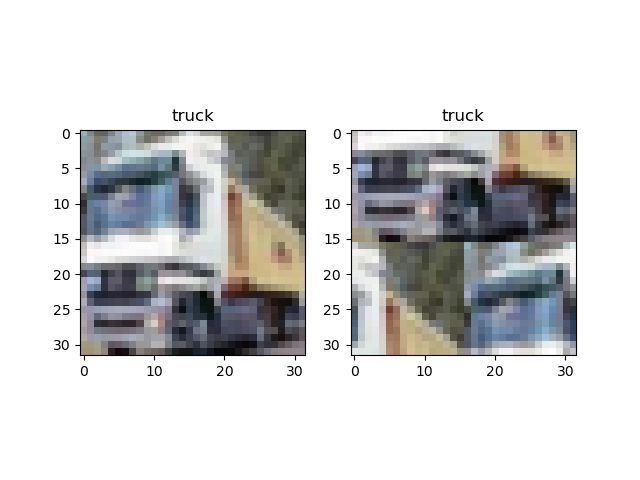
\includegraphics[width=0.45\textwidth]{shuffled image1.png}
    }
    \subfigure{
        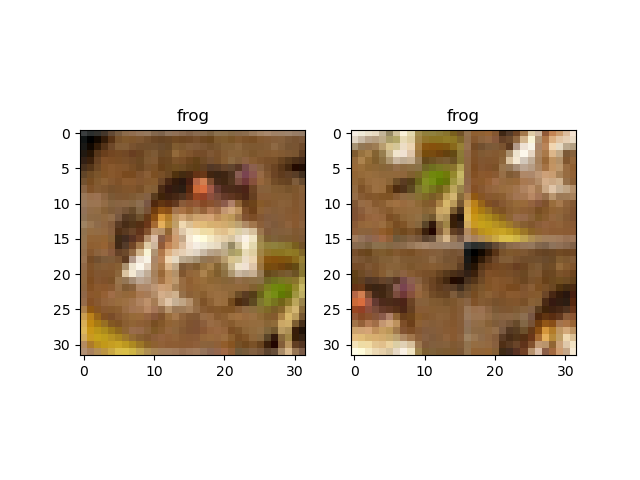
\includegraphics[width=0.45\textwidth]{shuffled image2.png}
    }
    \caption{打乱前后图像对比}
\end{figure}

\subsection{训练模型}
使用Adam优化算法训练模型,学习率为0.0001。定义损失函数为均方误差损失函数。训练50轮,每轮训练集训练一次,测试集测试一次。训练结果如下:

\begin{figure}[H]
    \centering
    \subfigure[DPN损失函数变化]{
        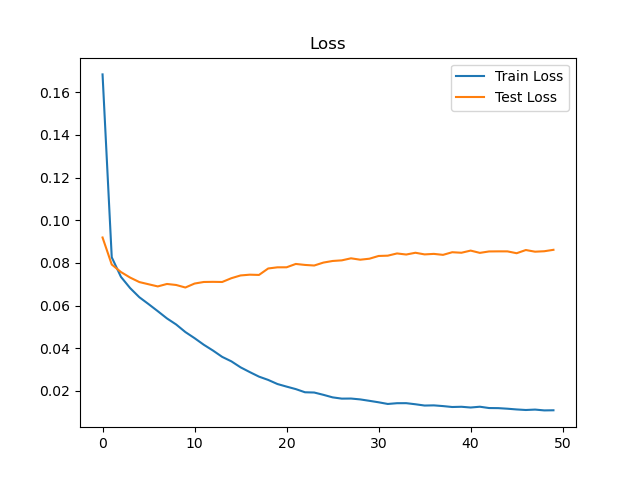
\includegraphics[width=0.4\textwidth]{Loss.png}
    }
    \subfigure[DPN准确率变化]{
        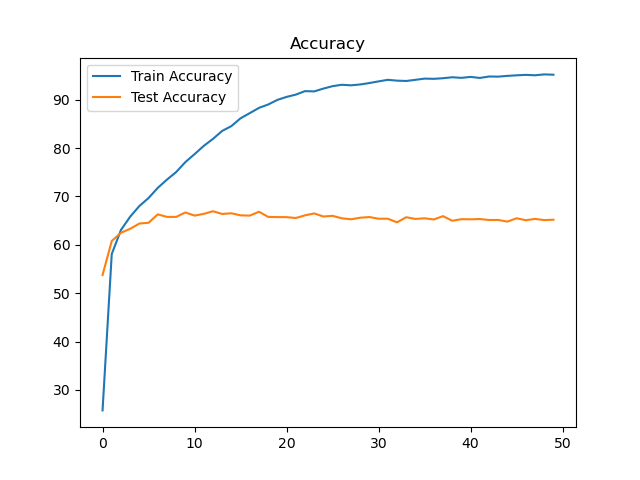
\includegraphics[width=0.4\textwidth]{Accuracy.png}
    }
    \caption{DPN训练结果}
\end{figure}
通过损失函数变换可以看出:在训练到第10轮左右后,测试集损失函数逐渐上升,训练集损失函数逐渐下降,说明模型出现了过拟合现象,模型在第10轮左右达到了最佳性能。故取第10轮的测试结果作为最终结果,测试集准确率约为66\%,模型对于分割为4份的图像复原效果较好。

\begin{figure}[H]
    \centering
    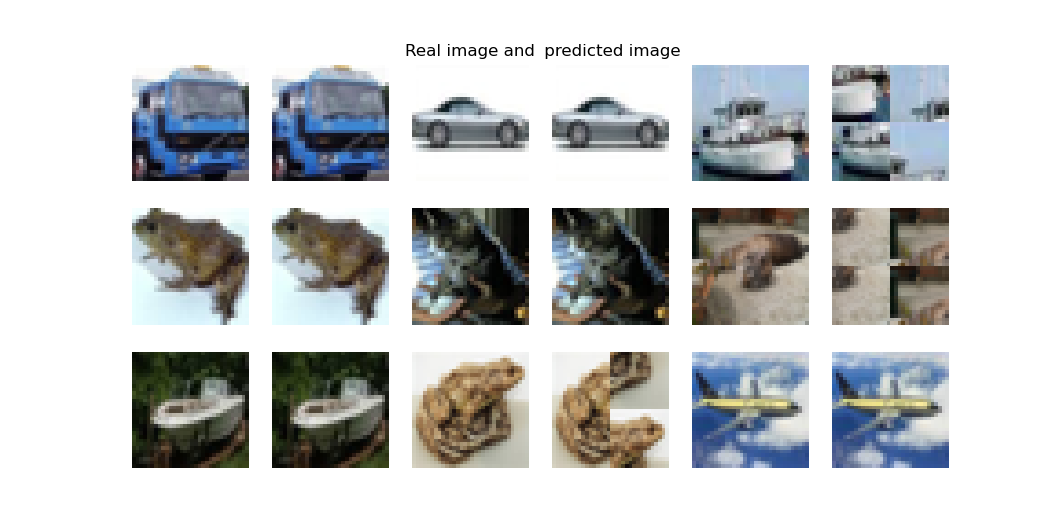
\includegraphics[width=0.8\textwidth]{recovered images.png}
    \caption{原始图像(左)与复原图像(右)对比}
\end{figure}

\end{document}